\documentclass[t]{beamer}
%%\usetheme{Szeged}
\usetheme{Antibes}
\usecolortheme{dolphin}
\usepackage{cmap}					%поиск в pdf
\usepackage[T2A]{fontenc}			% кодировка
\usepackage[utf8]{inputenc}			% кодировка исходного текста
\usepackage[english,russian]{babel}	% локализация и переносы
%%% Работа с картинками
\usepackage{graphicx}  % Для вставки рисунков
\graphicspath{{images/}{images2/}}  % папки с картинками
\setlength\fboxsep{3pt} % Отступ рамки \fbox{} от рисунка
\setlength\fboxrule{1pt} % Толщина линий рамки \fbox{}
\usepackage{wrapfig} % Обтекание рисунков текстом

%%% Работа с таблицами
\usepackage{array,tabularx,tabulary,booktabs} % Дополнительная работа с таблицами
\usepackage{longtable}  % Длинные таблицы
\usepackage{multirow} % Слияние строк в таблице

%%% Программирование
\usepackage{etoolbox} % логические операторы

%%% Другие пакеты
\usepackage{lastpage} % Узнать, сколько всего страниц в документе.
\usepackage{soul} % Модификаторы начертания
\usepackage{csquotes} % Еще инструменты для ссылок
%\usepackage[style=authoryear,maxcitenames=2,backend=biber,sorting=nty]{biblatex}
\usepackage{multicol} % Несколько колонок

%%% Картинки
\usepackage{tikz} % Работа с графикой
\usepackage{pgfplots}
\usepackage{pgfplotstable}

\title{Senty}
\author{Балакший Андрей \and Сухочев Александр 
	\and \newline Куратор:Юрий Курочкин}
\date{19 мая 2015}
\institute[Computer Science Center]

\begin{document}
	\frame[plain]{\titlepage}
	
	
	\section{О проекте}
	\begin{frame}
		\frametitle{\insertsection}
		\textbf{Поиск упоминаний и сентиментальная разметка коротких и 	очень коротких текстов(с использованием "чистой"\ разметки обучающего множества).}
	\end{frame}
	
	
	\section{Вдохновение}
	\begin{frame}
		\frametitle{\insertsection}
		\textbf{Прочитали статью ребят из Стэнфорда о сентиментальной разметке твитов. Ребята производили "грязную"\ разметку твитов(разметка по смайликам) и обучались по ней.}\pause
		
		\textbf{Захотелось чего-то аналогичного, но с русским языком и с "чистой"\ разметкой(разметкой вручную).}
	\end{frame}
	
	
	\section{Цель}
	\begin{frame}
		\frametitle{\insertsection}
		\textbf{Хотим по короткому тексту понимать настроение человека, написавшего его.}
	\end{frame}
	
	
	\section{Что планируем сделать}
	\begin{frame}
		\frametitle{\insertsection}
		\begin{itemize}
			\item Найти источник для обучения, содержащий высказывания людей на различные темы.	
			\item Придумать разнообразные фичи для текстов из нашего источника(признаки, которые помогут определять настроения людей, написавших данный текст) и реализовать по ним машинное обучение.
		\end{itemize}
	\end{frame}
	
	
	\section{Этапы выполнения}
	\subsection{Получение материала для обучения}
	\begin{frame}
		\frametitle{\insertsection}
		\framesubtitle{\insertsubsection}
		\textbf{Необходимо получить материалы для обучения.}\pause
		
		\textbf{Решение: \newline Парсим цитаты (далее называемые башами) с bash.im с помощью Beautiful Soup и сохраняем их в формате json.}
		
\includegraphics[scale = 0.8]{images/bash_im.png}
		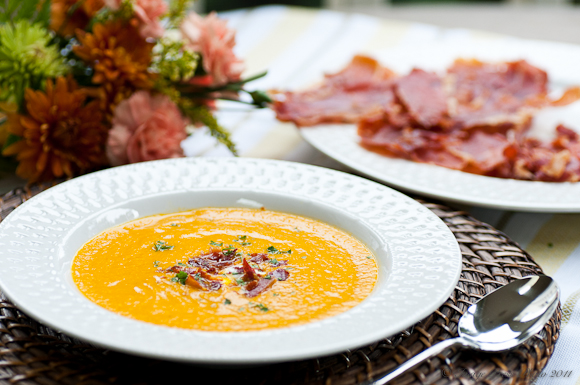
\includegraphics[scale = 0.3]{images/beautiful_soup.jpg}
	\end{frame}
	
	
	\subsection{Надо сделать чистую разметку}
	\begin{frame}
		\frametitle{\insertsection}
		\framesubtitle{\insertsubsection}
		\textbf{Как это лучше делать?}\pause
		\textbf{ Было принято решение написать приложение под android для чистой разметки на Java}\pause
		
		~~~~~~~
		{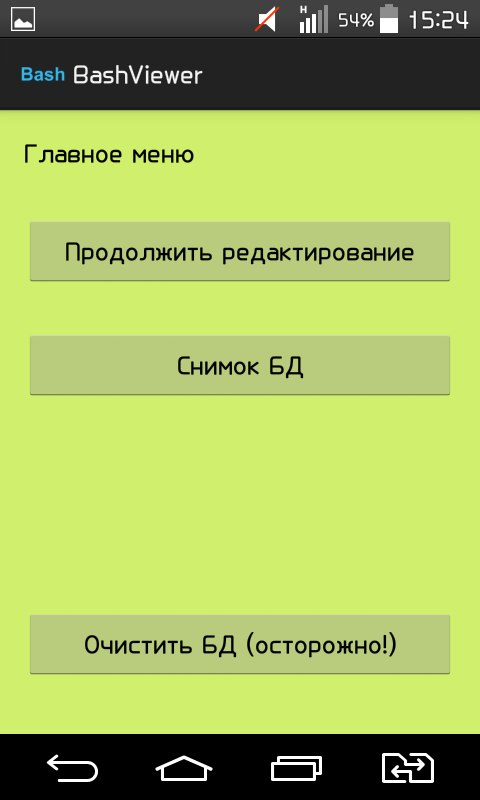
\includegraphics[scale = 0.17]{images/Bash1.jpg}
		
\includegraphics[scale = 0.17]{images/Bash2.jpg}
		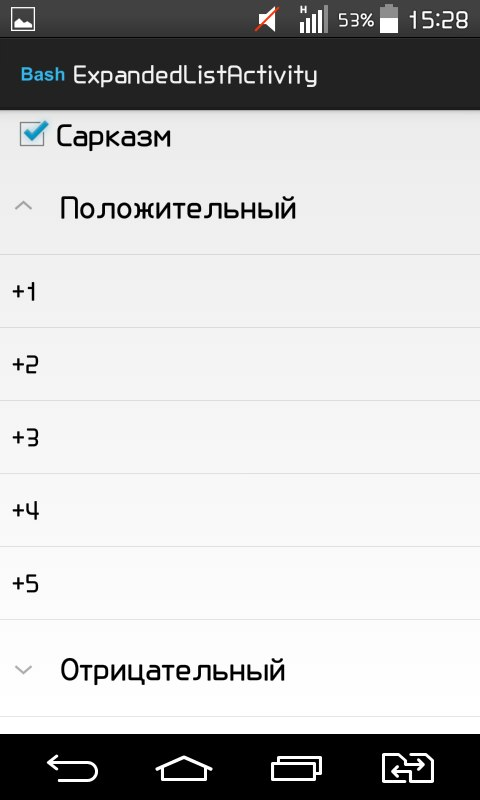
\includegraphics[scale = 0.17]{images/Bash3.jpg}}\pause	
	
		Отмечу, что хоть приложение и называется BashViewer, однако туда можно запихнуть тексты из любого источника. 
	\end{frame}

	\subsection{Выбор классификаторов}
	\begin{frame}
		\frametitle{\insertsection}
		\framesubtitle{\insertsubsection}
		
		\begin{itemize}
			\item 
			Naive Bayes
			\item
			SVM
			\item
			MaxEntropy			
		\end{itemize}\pause
		
		scikit-learn.org - спасибо, что ты есть!
		

	\end{frame}	
	
	\subsection{Экстрактор и фичи}
	\begin{frame}
		\frametitle{\insertsection}
		\framesubtitle{\insertsubsection}
		\textbf{Для выделения термов из башей был написан экстрактор, который выделял слова, отметая знаки препинания и прочие разделители, и приводил их к нормальной форме с помощью Mystem. Далее было придумано множество различных фич, которые представляли собой дополнительные опции экстрактора и отвечали за создание новых термов и удаление из рассмотрения уже существующих. Их можно использовать в различных комбинациях для повышения точности машинного обучения.}
	\end{frame}
	
	\subsection{Примеры работы различных фич}
	\begin{frame}
		\frametitle{\insertsection}
		\framesubtitle{\insertsubsection}
		
		\begin{itemize}
			\only<1-6>{\item \textbf{Исходный текст:} \newline "УЖАААСНО не люблю вставать по понедельникам и идти на работу ((((,... и по вторникам тоже ))"}
			
			\only<2-4>{\item \textbf{Работа стандартного экстрактора с Mystem:} \newline"ужааасно не любить вставать по понедельник и идти на работа (((( и по вторник тоже ))"}
			
			\only<3-4>{\item \textbf{Добавление фичи, убирающей предлоги, союзы и местоимения:} \newline "ужааасно не любить вставать понедельник идти работа (((( вторник тоже ))"}
			
			\only<4>{\item \textbf{Добавление фичи, убирающей повторные буквы:} \newline "ужасно не любить вставать понедельник идти работа (((( вторник тоже ))"}
			
			\only<5-6>{\item \textbf{Добавление фичи, склеивающей "не" со словом, которому эта частица принадлежит:} \newline "ужасно нелюбить вставать понедельник идти работа (((( вторник тоже"}
			
			\only<6>{\item \textbf{Добавление фичи, выделяющей смайлики:} \newline "ужасно нелюбить вставать понедельник идти работа \alert{плохосмайл} вторник тоже \alert{хоросмайл}"} 
		\end{itemize}
		
	\end{frame}
	
	\subsection{Структура проекта}
	\begin{frame}
		\frametitle{\insertsection}
		\framesubtitle{\insertsubsection}
		{Теперь нужно как-то объединить всё в одно целое.}\pause
		
		
		~
		
		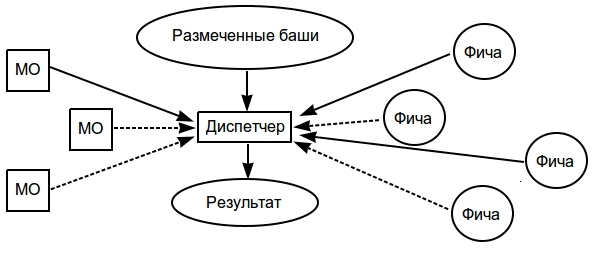
\includegraphics[scale=0.52]{images/TheManager.jpg}
	\end{frame}	
	
	
	\section{Проблемы}
	
	\begin{frame}
		\frametitle{\insertsection}
		\begin{itemize}
			\item{Малый объём выборки(примерно каждый четвёртый баш является эмоционально окрашенным, много сарказма, "чистая"\ разметка - дело не быстрое)}\pause
			\item{Сильный "перекос"\ в сторону отрицательных башей в обучающей выборке: из 1115 башей, имеющих эмоциональную окраску, 732 отрицательных (65.65 \%)}
		\end{itemize}
	\end{frame}

	\section{Дальнейшие перспективы}
	\begin{frame}
		\frametitle{\insertsection}
		\begin{itemize}
			\item
			{Двойная классификация: сначала классифицировать на нейтральное/с эмоциональной окраской, потом уже эмоциональные на положительные/отрицательные. }\pause
			\item
			{Прикрутить поиск по упоминаниям по базе башей для определения в скольких упоминаниях о предмете поиска отзывались положительно/отрицательно/нейтрально, с возможностью получения детальной информации по башам (по какому-то фильтру например)}\pause
			\item
			Увеличение материала для обучения 
			
		\end{itemize}
		
	\end{frame}
		
	
	\section{Итоги практики}
	
	
	\begin{frame}
		\frametitle{\insertsection}
		\begin{itemize}
			\item{Работа в команде}
			\item{Изучение Python(Mystem, Scikit learn, Beautiful soup)}
			\item{Работа с GitHub}
			\item{Работа с \LaTeX}
		\end{itemize}
		~~~~~~~~~
		
\includegraphics[scale = 0.08]{images/git_hub.png}
		
\includegraphics[scale = 0.08]{images/latex-logo.png}
		
\includegraphics[scale = 0.2]{images/scikit_learn.png}
	\end{frame}
	
	
	
	
	\section{Спасибо за внимание}
	
	\begin{frame}
		\frametitle{\insertsection}
		\href{https://github.com/cscenter/senty}{https://github.com/cscenter/senty}
	\end{frame}
	
	
	
	
	
	
	
	
	
	
\end{document}